\documentclass{article}

\usepackage{amsmath}
\usepackage{amssymb}
\usepackage{amsfonts}
\usepackage{mathtools}

\usepackage{graphicx}

\usepackage[thmmarks, amsmath]{ntheorem}

\usepackage{diffcoeff}
\diffdef{}{op-symbol=\mathrm{d},op-order-sep=0mu}
\usepackage{cancel}

\usepackage{enumitem}

\setlist{label=\alph*)}

\title{Differential Geometry Homework 3}
\author{Duarte Maia}
\date{}

\theorembodyfont{\upshape}
\theoremseparator{.}
\newtheorem{ex}{Exercise}

\theoremstyle{nonumberplain}
\theoremheaderfont{\itshape}
\theorembodyfont{\upshape}
\theoremseparator{:}
\theoremsymbol{\ensuremath{\blacksquare}}
\newtheorem{sol}{Solution}

\newcommand{\R}{\mathbb{R}}
\newcommand{\C}{\mathbb{C}}
\newcommand{\Z}{\mathbb{Z}}

\newcommand{\PP}{\mathbb{P}}
\newcommand{\FF}{\mathcal{F}}

\newcommand{\I}{\mathrm{i}}
\newcommand{\e}{\mathrm{e}}


\DeclareMathOperator{\inte}{int}
\DeclareMathOperator{\codim}{codim}
\DeclareMathOperator{\Lie}{Lie}
\DeclareMathOperator{\Ad}{Ad}
\DeclareMathOperator{\ad}{ad}
\newcommand{\grad}{\nabla}

\DeclarePairedDelimiter{\norm}{\lvert}{\rvert}

\begin{document}
\maketitle

\begin{ex}
Give an example of a one-dimensional distribution which is not globally generated by a vector field.
\end{ex}

\begin{sol}
Consider the (open) Möbius strip, given by a square with the left and right side identified with opposite orientations. Then, the `vertical distribution' is not globally generated. To show this, we may cover the Möbius strip into two rectangular charts such as in the following figure:

\begin{center}
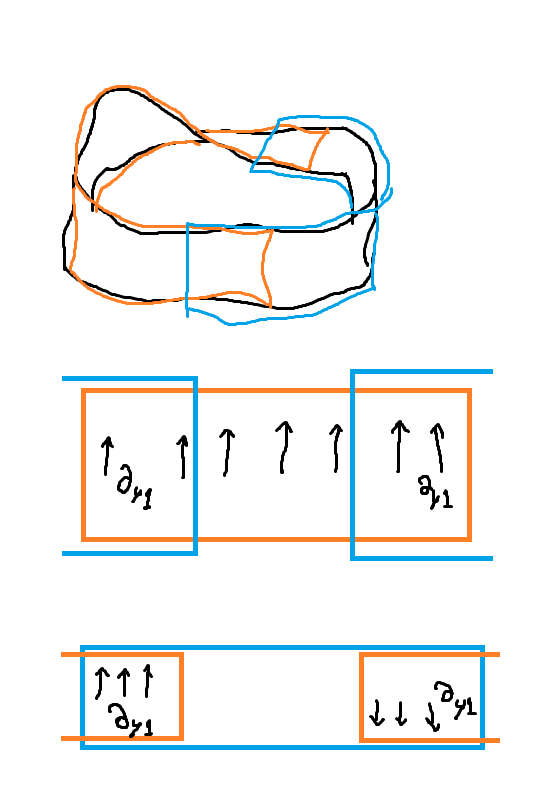
\includegraphics[width=.7\linewidth]{mobcharts}
\end{center}

We use $\partial_{y1}$ to represent the coordinate $y$ vector in the orange chart, and $\partial_{y2}$ to represent the coordinate $y$ vector in the blue chart. The important thing to note is that the charts intersect at two rectangles. In one of them, $\partial_{y1} = \partial_{y2}$, while in the other $\partial_{y1} = - \partial_{y2}$.

Now, the distribution at hand is locally generated by these coordinate $y$ vectors. However, it cannot be globally generated. Indeed, if $X$ were a vector field that globally generated the vertical distribution, then over the orange chart it would have to be of the form $f \partial_{y1}$, where $f$ is never null, and therefore could never change sign because the orange chart is connected. A similar argument shows that over the blue chart $X$ would be of the form $g \partial_{y2}$, where $g$ never changes sign. But this yields a contradiction, because over the intersection $X$ must be of the form
\[f \partial_{y1} = g \partial_{y2},\]
where $f$ and $g$ never change signs. If we look at the section where $\partial_{y1} = \partial_{y2}$ we conclude that the signs of $f$ and $g$ must be the same, but if we look at the section where $\partial_{y1} = - \partial_{y2}$ their signs must be opposite. This contradiction proves that the vector field $X$ cannot exist.
\end{sol}

\begin{ex}
Let $G$, $H$ be connected Lie groups and $\phi \colon G \to H$ a smooth homomorphism. Suppose that $(\dl \phi)_e$ is an isomorphism. Show that $\phi$ is a covering map.
\end{ex}

\begin{sol}
Since $(\dl \phi)_e$ is an isomorphism, there exists a neighborhood of the identity, say $U \subseteq G$, such that $\phi$ is a diffeomorphism from $U$ to $\phi(U)$. Consequently, for any $g \in G$ there exists a neighborhood $g U$ of $g$ such that $\phi$ is a diffeomorphism from $g U$ to $\phi(g) \phi(U)$, which is a neighborhood of $\phi(g)$.

Now, as a consequence, for any $h \in H$ for each $g \in \phi^{-1}(g)$ there exists a neighborhood $g U$ of $g$ such that $\phi$ is a diffeomorphism from $g U$ to a (common) neighborhood of $h$, namely $h \phi(U)$. If all the $g U$ were disjoint, they would form a decomposition of $\phi^{-1}(h \phi(U))$, and so we would be very close to proving that $\phi$ is a covering map, the only remaining property to check being that $\phi$ is surjective.

We will now show that all the $g U$ are disjoint. Indeed, suppose that some $g_1 U$ intersected some $g_2 U$, with $\phi(g_1) = \phi(g_2)$. By multiplying both sets by $g_1^{-1}$, we may in fact assume that $g_1 = e$, that is: We assume for the sake of contradiction that $U$ intersects $g U$ for some $g \neq e$ satisfying $\phi(g) = e$. This is to say that there exist $u_1, u_2 \in U$ such that $u_1 = g u_2$. Taking $\phi$ on both sides, one obtains that $\phi(u_1) = \phi(u_2)$, and since both $u_i$ are in $U$, on which $\phi$ is injective, we conclude $u_1 = u_2$ and so $g = e$, a contradiction. This concludes the proof that all $gU$ are disjoint, and with it the proof of the `stack of pancakes' condition, for we have decomposed $\phi^{-1}(h \phi(U))$ into a disjoint union of opens restricted to which $\phi$ is a diffeomorphism onto $h \phi(U)$.

We now prove that $\phi$ is surjective. Let $h \in H$. Since $H$ is connected, there exists a smooth path $\gamma$ which goes from the identity to $h$ (at time 1, say). Define $v(t) = (\dl L_{\gamma(t)^{-1}}) \dot\gamma(t)$, and set $w(t) = (\dl \phi)_e^{-1}(v(t))$. Finally, define $\eta(t)$ as the solution to the following ODE:
\[
\begin{cases}
\eta(0) = e,\\
\dot\eta(t) = (\dl L_{\eta(t)}) w(t).
\end{cases}
\]

The fact that this ODE has solution up to time 1 deserves some explanation. Suppose that the solution exists only until some time $T < 1$. Then, let $\sigma(t)$ be the solution of the same ODE, but with initial conditions $\sigma(T) = e$. Then, we may glue a translate of $\sigma$ to increase the domain of $\eta$ as follows. Let $t_0 < T$ be some time that is both in the domain of $\sigma$ and the domain of $\eta$. Then, define $\theta(t) = \eta(t_0) \sigma(t_0)^{-1} \sigma(t)$. The idea is that since the ODE is left-invariant, left translations only change the initial conditions, and so we conclude that both $\theta$ and $\eta$ are solutions to the ODE
\[
\begin{cases}
\theta(t_0) = \eta(t_0),\\
\dot\theta(t) = (\dl L_{\theta(t)}) w(t).
\end{cases}
\]

By uniqueness of solution, since $\theta$ exists up to and beyond time $T$, so must $\eta$, which is a contradiction with the hypothesis that it did not.


Now that we have shown that $\eta(1)$ exists, we will prove that $\phi(\eta(1)) = h$. To do so, we consider the pushforward of the path $\eta$, which satisfies $\phi(\eta(0)) = e$, and furthermore
\begin{multline*}
\diff{}t \phi(\eta(t)) = (\dl \phi) \dot\eta(t) = (\dl \phi)(\dl L_{\eta(t)}) w(t)\\
= (\dl L_{\phi(\eta(t))}) (\dl \phi) w(t) = (\dl L_{\phi(\eta(t))}) v(t).
\end{multline*}

In other words, $\phi(\eta(t))$ is the solution to the ODE with initial conditions at $e$ and with velocity given by the left-invariant vector field generated by $v(t)$. But by definition of $v(t)$, the original path $\gamma$ was also a solution to this ODE, and so we conclude $\phi(\eta(t)) = \gamma(t)$ and therefore $\phi(\eta(1)) = \gamma(1) = h$. This concludes the proof of surjectivity.

\smallskip

(Note: Meanwhile I found an alternate proof, which is probably the intended solution. Any element of $H$ can be written as a product of exponentials, say $h = \exp(A_1) \exp(A_2) \dots \exp(A_n)$, so we define $B_i = (\dl \phi)^{-1}(A_i)$ and consider $g = \exp(B_1) \dots \exp(B_n)$. Naturality of the exponential immediately yields $\phi(\exp(B_i)) = \exp(A_i)$ and consequently $\phi(g) = h$.)
\end{sol}

\begin{ex}
Let $\psi \colon G \times M \to M$ be a smooth left action. For $A \in \Lie(G)$, define
\[X_A = \diff{}t[0] (\exp(tA) \cdot p).\]

Show that $[X_A, X_B] = - X_{[A,B]}$.
\end{ex}

\begin{sol}
We begin by considering an alternative, but obviously equivalent, definition for $X_A$:
\[(X_A)_p = (\dl h_p) A\text{, where $h_p(g) = g \cdot p$.}\]

With this in mind, we may calculate $(X_A)_p \cdot f$ explicitly, for $f \colon M \to \R$:
\[(X_A)_p \cdot f = (\dl h_p) A \cdot f = A \cdot (f \circ h_p).\]

Consequently, we obtain the following expression for a composite derivative:
\[(X_B)_p \cdot (X_A \cdot f) = (X_B)_p \cdot (q \mapsto A \cdot (f \circ h_q)) = B \cdot (g \mapsto A \cdot (f \circ h_{gp})),\]
and this expression can be simplified by noticing that
\[h_{gp}(g') = g' g p = (h_p \circ R_g)(g'),\]
and therefore
\begin{align*}
(X_B)_p \cdot (X_A \cdot f) &= B \cdot (g \mapsto A \cdot (f \circ h_{p} \circ R_g))\\
&= B \cdot (g \mapsto (\dl R_g) A \cdot (f \circ h_{p}))\\
&= B \cdot RA \cdot (f \circ h_p),
\end{align*}
where $RA$ is the \emph{right}-invariant vector field generated by $A$. As a consequence,
\[ [X_A, X_B]_p \cdot f = X_{[RA,RB]_e} \cdot f,\]
so it only remains to relate the `right-invariant Lie bracket' with the usual one.

To this effect, let us calculate $A \cdot (RB \cdot f))$, where $f$ is an arbitrary function $G \to \R$. We may write this out in terms of derivatives and exponentials:
\[A \cdot (RB \cdot f) = \diff{}t[0] (RB \cdot f)(\exp(tA)) = \diff{}t[0] \diff{}s[0] f(\exp(sB) \exp(tA)),\]
and now, since this is a derivative of a function from $\R^2$ to $\R$, we may exchange the order of differentiation to obtain
\[A \cdot (RB \cdot f) = \diff{}s[0] \diff{}t[0] f(\exp(sB) \exp(tA)) = \diff{}s[0] (LA \cdot f)(\exp(sB)) = B \cdot (LA \cdot f),\]
where $LA$ is the left-invariant vector field associated to $A$.

From this computation, it is very easy to conclude by expanding $[A,B] \cdot f$ that
\[ [RA,RB]_e = [B,A] = -[A,B].\]

Finally, using the fact (obvious from the definition that we presented at the start of the solution) that the $X$ operator is linear, we obtain
\[[X_A, X_B] = X_{[RA,RB]_e} = -X_{[A,B]},\]
as we desired to show.
\end{sol}

\begin{ex}
Suppose that the action in the above exercise is a right action. What happens to the induced infinitesimal action?
\end{ex}

\begin{sol}
The only thing that would change in the proof would be that we should define $h_p(g) = pg$ instead of $h_p(g) = gp$, so the identity $h_{gp} = h_p \circ R_g$ would be swapped into
\[h_{gp} = h_p \circ L_g.\]

Consequently, where we previously obtained $[X_A, X_B] = X_{[RA,RB]_e}$, we now obtain $[X_A, X_B] = X_{[LA,LB]_e}$, and therefore,
\[[X_A,X_B] = X_{[A,B]}.\]

In other words, the induced infinitesimal action would be a Lie algebra homomorphism, rather than an antihomomorphism.
\end{sol}

\begin{ex}
Define $\Ad_g(A) = \diff{}t[0] g \exp(tA) g^{-1}$.

\begin{enumerate}
\item Show that $\Ad_g \circ \Ad_h = \Ad_{gh}$.
\item Let $\ad(A)(B) = \diff{}t[0] \Ad_{\exp(tA)} B$. Show that $\ad(A)(B) = [A,B]$.
\end{enumerate}
\end{ex}

\begin{sol}
a) First, we remark that $\exp(tA)$ in the definition of $\Ad$ can be replaced by any curve $\alpha$ such that $\dot\alpha(0) = A$, as is evident by the definition given in terms of the derivative of conjugation by $g$.

Next, note that by definition the curve
\[\gamma(t) = g \exp(tA) g^{-1}\]
is a curve whose derivative at zero is equal to $\Ad_g(A)$. Consequently, we may write
\[\Ad_h(\Ad_g(A)) = \diff{}t[0] h \gamma(t) h^{-1},\]
and expanding the definition of $\gamma$ one easily concludes that
\[\Ad_h(\Ad_g(A)) = \Ad_{hg}(A),\]
as we desired to show.

\medskip

b) Let us compute $\ad(A)(B)$ by applying it to some function $f \colon G \to \R$.
\begin{align*}
\ad(A)(B)\cdot f &= \diff{}t[0] \Ad_{\exp(tA)}B \cdot f\\
&= \diff{}t[0] \diff{}s[0] f(\exp(tA) \exp(sB) \exp(-tA)).
\end{align*}

Now, these are `old-school derivatives' of a function which goes from $\R^2$ to $\R$, whose variables are $t$ and $s$. Consequently, we may interchange the order of differentiation, and we now focus on the term
\[\diff{}t[0] f(\exp(tA) \exp(sB) \exp(-tA)).\]

This derivative can be simplified using the following formula, which is an easy consquence of the chain rule. If $F \colon \R^2 \to \R$ is differentiable,
\[\diff{}t[0] F(t,t) = \partial_1 F(0,0) + \partial_2 F(0,0).\]

Consequently,
\begin{multline*}
\diff{}t[0] f(\exp(tA) \exp(sB) \exp(-tA))\\
= \diff{}t[0] f(\exp(tA) \exp(sB)) + \diff{}t[0] f(\exp(sB) \exp(-tA)).
\end{multline*}

We may now simplify these terms. We begin with the second one, $\diff{}t[0] f(\exp(sB) \exp(-tA))$. It is clearly the application to $f$ of the vector $(\dl L_{\exp_(sB)}) (-A)$, or in other words, if we identify a vector with the left-invariant vector field associated to it,
\[\diff{}t[0] f(\exp(sB) \exp(-tA)) = (-A \cdot f)(\exp(sB)).\]

Now, taking the derivative in $s$, one clearly obtains the term $-B \cdot (A \cdot f)$.

the other term, that is $\diff{}t[0] f(\exp(tA) \exp(sB))$, can be similarly simplified, but one must first take the derivative in $s$ and interchange the derivatives. Once one does, though, one obtains a similar result, of $A \cdot (B \cdot f)$. In conclusion, the original derivative has been simplified to
\[\ad(A)(B)\cdot f = A \cdot (B \cdot f) - B \cdot (A \cdot f) = [A,B] \cdot f,\]
which proves the desired result.

\end{sol}

\end{document}